\section[Overview]{Overview
\footnote{
  $CVS~revision~ $Id: hrs-1999.tex,v 1.1 2003/06/06 15:44:08 gen Exp $ $ 
}
\footnote{Authors: J.LeRose \url{mailto:lerose@jlab.org}}
}
   
The Hall A spectrometers and associated instrumentation are designed to 
perform high resolution and high accuracy experiments.  The goal is to 
achieve a missing mass resolution of $\sim$ 200-500 keV to clearly 
identify the nuclear final state.  An absolute accuracy of $\sim$ 1\% is 
also required by the physics program planned in the Hall, which implies 
$\sim$ 10$^{-4}$ accuracy in the determination of particle momenta and 
$\sim$ 0.1 mr in the knowledge of the scattering angle.

The instruments needed are a high resolution electron spectrometer 
(HRES) and a high resolution hadron spectrometer (HRHS), both with a 
maximum momentum capability matching the TJNAF beam energy, and large 
angular and momentum acceptance.

\begin{figure}[tbp]
\begin{center}
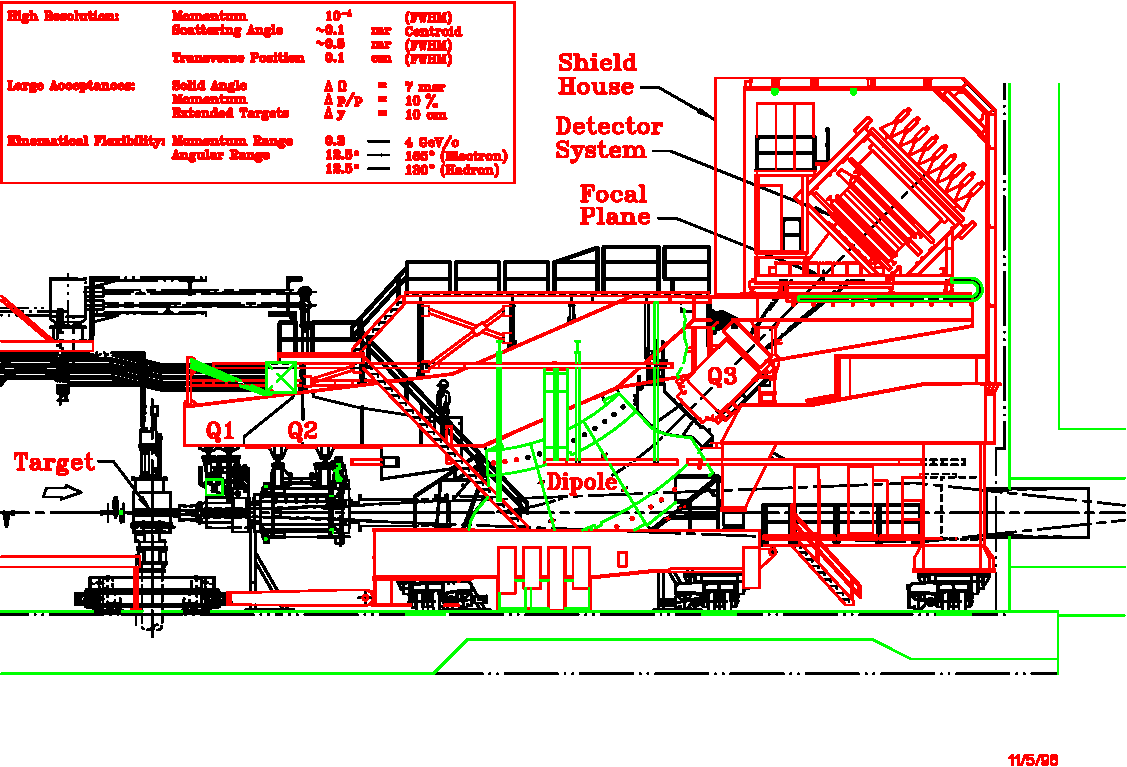
\includegraphics[angle=0,width=\textwidth,clip]{figure0101_r}
{\linespread{1.}
\caption[Spectrometers: Elevation View of Hall~A HRS]{A side view of the Hall~A
HRS spectrometer.}  
\label{fig:hrs_ev}}
\end{center}
\end{figure}
 
\begin{figure}[tbp]
\begin{center}
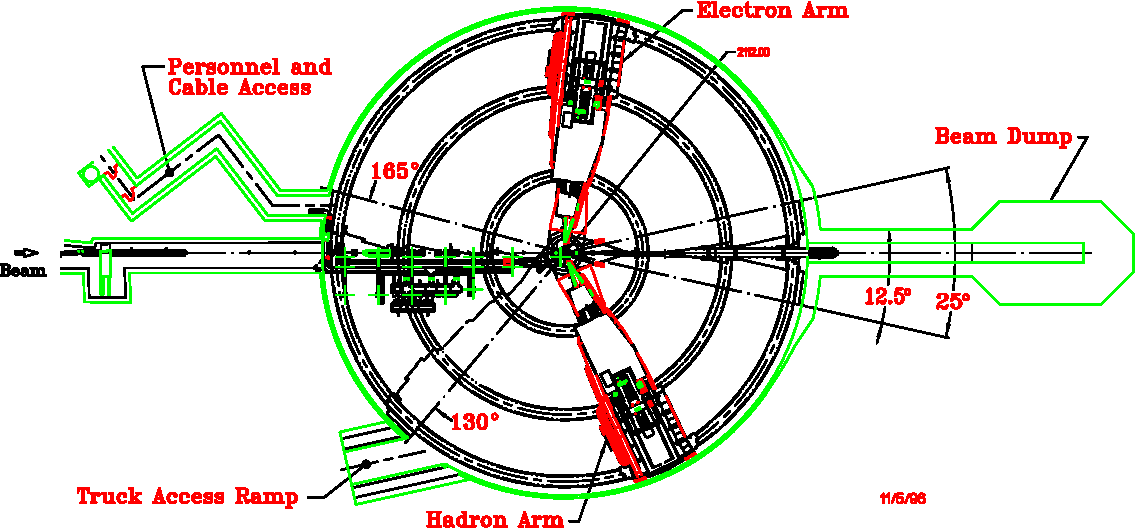
\includegraphics[angle=0,width=\textwidth,clip]{figure0102_r}
{\linespread{1.}
\caption[Spectrometers: Plan View of Hall~A]{A bird's eye view of the Hall~A
end-station at TJNAF.}  
\label{fig:hrs_pv}}
\end{center}
\end{figure}


A layout of the 4 GeV/c High Resolution Electron Spectrometer is shown 
on Figures~\ref{fig:hrs_pv} and \ref{fig:hrs_ev}.
Its main design characteristics are 
given in the attached table.  The spectrometer has a vertical bending 
plane and 45$^{\circ}$ bending angle.  The QQDQ design includes four 
independent superconducting magnets, three current-dominated 
cos2$\theta$ quadrupoles and one iron-dominated dipole with 
superconducting racetrack coils.  The second and third quadrupoles of 
each spectrometer have sufficiently similar field requirements that they 
are of identical design and construction.  The overall optical length, 
from target to focal plane, is 23.4 m.  Optically, the HRHS 
is essentially identical to HRES. In fact the two spectrometers can be used 
interchangeably to detect either positively or negatively charged particles 
as needed by any particular experiment. 

The support structure includes all system elements which bear the weight 
of the various spectrometer components and preserve their spatial 
relationship as required for 45$^{\circ}$ vertical bending optics.

The alignment and positioning system includes all the elements which 
measure and adjust the spatial relationship.  The support structure 
consists of the fabricated steel components which support the magnets, 
detector, shield house and associated equipment.  It is composed of the 
box beam, which supports the outer elements in fixed relative position 
atop the dipole; the dipole support bracket, upon which the dipole rests on 
the jacks; the cradle, upon which the dipole rests through the vertical 
positioning system, VPS; and a portion of the shield house load through 
the inboard legs of the gantry; the gantry, which supports the shield 
house and the magnet power supplies; and the bogies, which support the 
cradle-gantry assembly and slide on the floor plates and provide the 
driving power to move the two spectrometer arms.

The detector package is supported on the box beam and is surrounded by 
the shield house.  It must perform two functions, tracking and particle 
identification, PID.  The most important capability of focusing 
spectrometers is measuring precisely the momenta and entrance 
orientations of the tracks.  Momenta resolution of 10$^{-4}$ is 
obtainable, consistent with the resolution of the incident beam.

A particle traversing the detector stack 
(Figure~\ref{fig:hrs_electron_det}) encounters two sets of horizontal 
drift chambers (x,y) with two planes of 368
wires in each chamber. The track resolution is $\sim$ 100 $\mu$m.  
From the chamber information both 
positions and angles in the dispersive and transverse directions can be 
determined.  The information from these chambers is the principal input 
of the tracking algorithms.

The chambers are followed by a scintillator hodoscope plane designated S1. 
This plastic scintillator array provides the timing reference for 
the drift chambers, and is also used in trigger formation and in combination 
with a second hodoscope pair it can provide time of flight particle 
identification.  These scintillators can also be used to perform crude 
tracking.

The next element encountered by a particle is a gas threshold Cerenkov 
detector.  This is used for particle identification.  In the hadron 
spectrometer this gas threshold Cerenkov detector can be swapped 
against an Aerogel detector, with a similar function.

The second hodoscope plane, S2, is located directly behind the 
gas Cerenkov.  Its function is essentially the same as that of S1.  
In the hadron spectrometer an option exists to have this hodoscope 
pair be preceded by a third chamber, to improve tracking.
 Each of the two spectrometers 
have gas and Aerogel Cerenkov detectors which can be used
 when they are in electron detection mode.

The final elements in the detector stack on HRSE are 
the pre-shower and the lead glass shower 
calorimeter.  This is used for energy determination and PID.

\begin{figure}[tbp]
\begin{center}
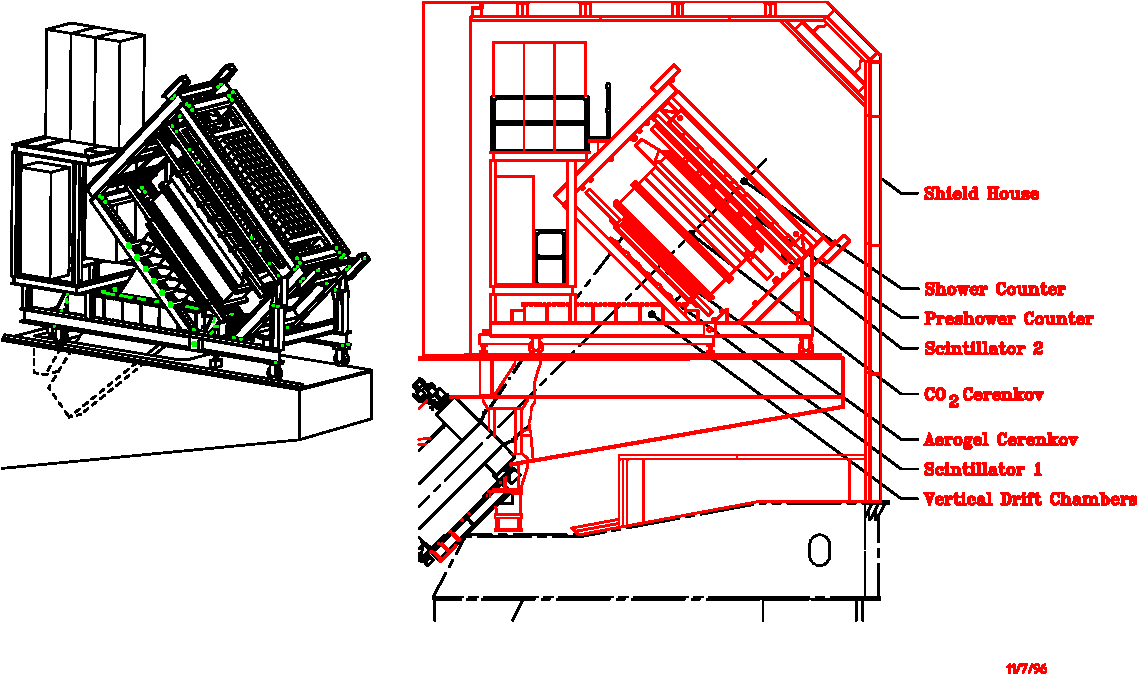
\includegraphics[angle=0,width=\textwidth,clip]{figure0103_r}
{\linespread{1.}
\caption[Spectrometers: Electron Arm Detectors]{The electron spectrometer detector stack.}
\label{fig:hrs_electron_det}}
\end{center}
\end{figure}

\begin{figure}[tbp]
\begin{center}
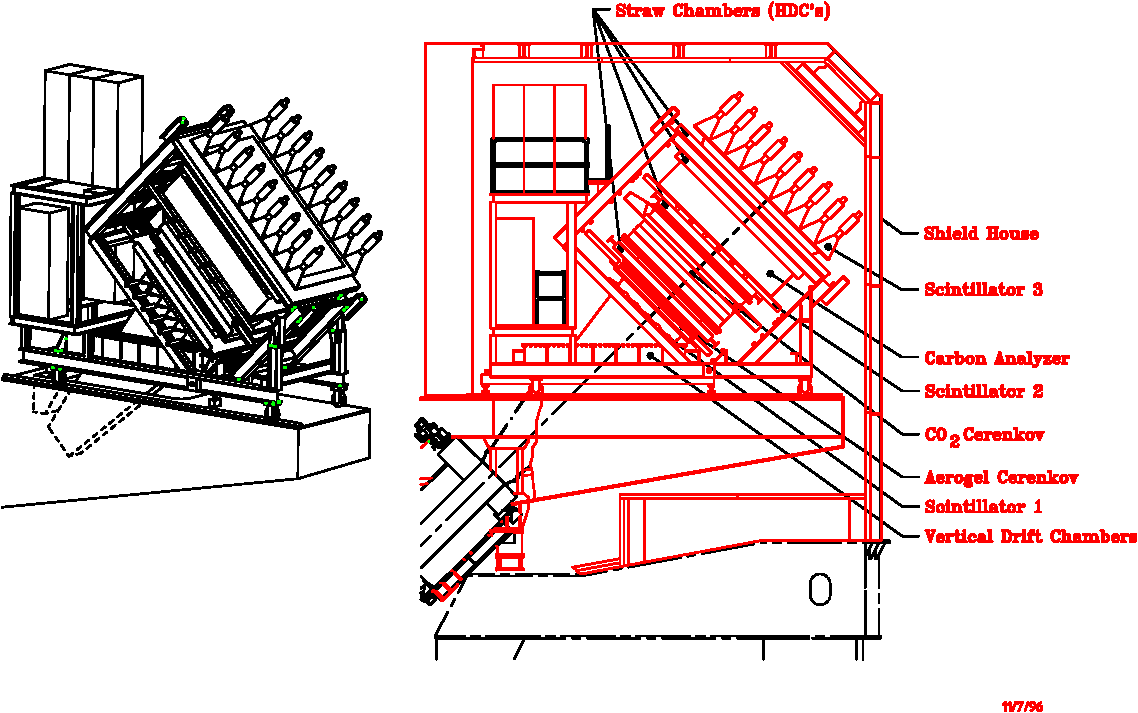
\includegraphics[angle=0,width=\textwidth,clip]{figure0104_r}
{\linespread{1.}
\caption[Spectrometers: Hadron Arm Detectors]{The hadron spectrometer detector stack.}
\label{fig:hrs_hadron_det}}
\end{center}
\end{figure}


The hadron detector is shown schematically in 
Figure~\ref{fig:hrs_hadron_det}.  It consists 
of two sets of (x,y) vertical drift chambers identical to those of the 
electron arm.  The remaining part of the detection system is used to 
define the level 1 trigger, as well as for particle identification and 
timing.  It consists of three minimally segmented planes of 
scintillation counters equipped with photomultipliers at both ends, and 
it includes Cerenkov counters (gas CO$_2$ and Aerogel).

In addition, a proton polarimeter is installed in the back of the 
detector package to measure the polarization of the proton using a 
segmented carbon analyzer up to 60 cm in thickness to allow measurements 
over a wide range of proton energies.  A pair of front and a pair of 
rear straw chambers determine the incident and 
scattered angles, respectively.  The third scintillation counter, 
located at the rear end, provides the trigger for the polarimeter.  The 
polarimeter detectors are dimensioned to accept a 20$^{\circ}$ cone of 
scattered protons.

Several support systems are necessary in addition to the basic 
components mentioned above.  They include gas supply systems for the 
wire chambers, high voltage supplies, readout electronics, a second 
level trigger, software for data analysis and testing, and a remotely 
controllable mechanical system.

As for the electron spectrometer, all detectors are mounted on a 
single rigid carriage along with their associated electronics.  The FPP 
components are mounted on an FPP subframe for installation and removal as 
a unit.  The trigger electronics are located next to the detectors, 
as for the electron arm.

To reduce the resolution degrading effects of multiple scattering, the 
entire interior of the spectrometer from the pivot to the detector hut 
is a vacuum vessel.  The ends of this evacuated volume are capped by 
relatively thin vacuum windows.

As mentioned, subsystems will be discussed in more detail in the next 
three sections.  The remainder of this section will describe some 
features common to the two spectrometers, then the following major 
sections will be devoted to the specifics that are not common.


\subsection{Safety with Regards to the Spectrometer}

The principle concern with the spectrometers is that they are large, 
and have associated vacuum, hydraulic, cryogenic and magnet systems all of 
which can be potentially dangerous.

The bogies which move the massive 1200 ton spectrometers must be 
carefully operated.  Inspection of the wheels to ensure there is no 
debris which the wheels could ride over is mandatory.  Similarly 
personnel need to be aware that the spectrometers are moving so that no one 
inadvertently gets trapped.

The vacuum systems associated with the spectrometers are essentially 
pressure vessels.  Care should be exercised so as not to puncture the 
windows.

The magnets themselves are installed inside cryostats.  These vessels 
are exposed to high pressures and are therefore equipped with safety 
relief valves and burst discs.

The hydraulic system that operates the vertical positioning system VPS 
and the horizontal positioning system HPS operates at high pressure, 
3000 - 5000 psi.  Therefore one should be careful when operating those 
systems.

The cryogenic system operates at elevated pressure at 4K.  One must 
guard against cold burns and take the normal precautions with pressure 
vessels when operating this system.  Only WBS7 are permitted to install 
and take out U tubes.

The magnets have a great deal of stored energy as they are large 
inductors. Always make sure people are clear of them and that
the dump resistor is attached to the magnet.

There are several major safety concerns with regards to the detectors, 
namely 1) flammable gas located in the VDC and FPP, 2) ODH hazard due to 
CO$_2$ in the Cerenkov counter, 3) high voltage due to the photo 
multipliers on the various detectors and 4) a thin vacuum window 
separating the detector array from the vacuum system in the 
spectrometers.  The clean agent fire suppression system, while installed 
to suppress fires, can also be a safety hazard.  It is possible for an 
individual to drop down alongside the box beam to the gantry roof 
inside the shield house.  This area, although technically not a confined 
space, could conceivably become one in the event that the clean agent 
system was attached.  Personnel should have a 5 minute air pack with 
them in the event they must enter the area alongside the box beam to the gantry roof 
inside the shield house.

\subsection{Hall A Vacuum System}

The Hall A vacuum system consists of 5 separate but interconnected 
subsystems.  The largest is designed to supply the Hall A HRS with a 
self contained 5 $\times$ 10$^{-6}$ Torr vacuum that enables both 
spectrometers to be pumped down from atm. in a few hours.  The target 
vacuum system is designed to maintain a 1 $\times$ 10$^{-6}$ Torr in 
order to minimize contamination and provide an insulating vacuum for the 
cryo target.  Rough insulating vacuum for the 4 superconducting magnets 
is provided by a 360 $cfm$ Roots type blower that can be connected to each 
magnet.  The beam line vacuum is maintained by 1 $\ell$/s ion pump 
system used in the accelerator ring and a small turbo pump located near 
the target.  The final subsystem is a differential pumping station 
located near the target exit port.

\subsubsection{Spectrometer Vacuum System}

The spectrometer vacuum system is shown in Figure~\ref{fig:hrs_vac_sys}.
Vacuum for the HRS is supplied by an Alcatel 880 $\ell$/s Turbo 
pump backed by a Balzers 360 $cfm$ Roots type Blower.  This Blower, via a 
special manifold, also supplies the roughing vacuum to the HRS at the 
Dipole Inlet Transition.  The first Turbo is mounted on the lower side 
of the Dipole entrance transition.  The roughing port is also located on 
this transition, on the top side.  The upper turbo is located on the 
lower side of the window transition.

Vacuum readouts and interlock outputs are supplied by five (5) HPS 
series 421 Cold Cathode gauges and seven (7) series 275 Mini-Convectron 
gauges.  In addition to these there will also be a FIsons Micromass 386 
RGA head installed in the system for diagnostic purposes.  Most of this 
instrumentation will be located on the Turbo pump manifold (for detailed 
information see Figure~\ref{fig:hrs_vac_sys}).

\begin{figure}
\begin{center}
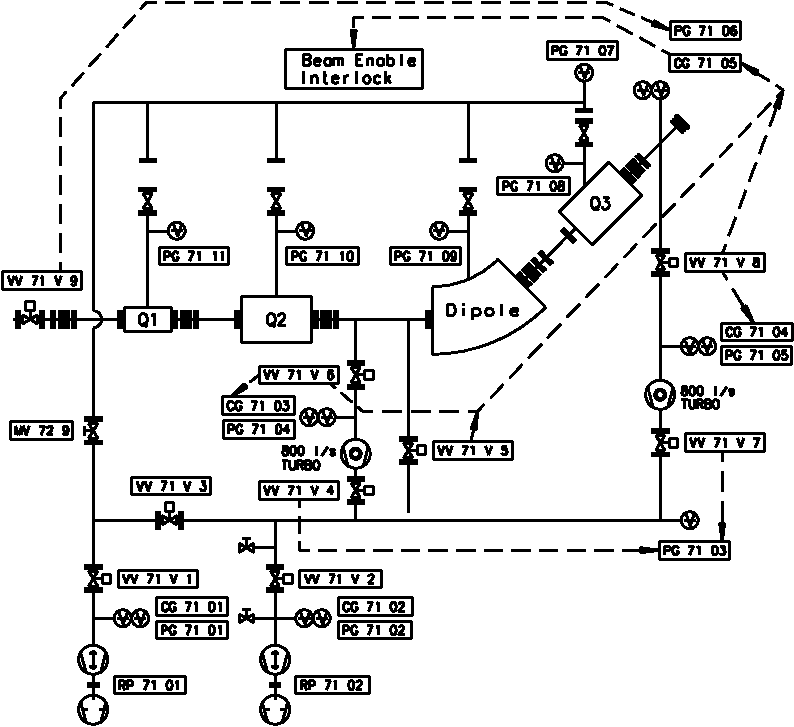
\includegraphics[angle=0,width=15cm]{fig0125new}
{\linespread{1.}
\caption[Spectrometers: HRS Vacuum System]{HRS vacuum system.}
\label{fig:hrs_vac_sys}}
\end{center}
\end{figure}

Powered valves, instrumentation and pumps will be controlled and powered 
at the Vacuum System equipment rack located on each respective 
spectrometer on the gantry platform.  Selective equipment will also be 
controllable from the Hall A counting house.

{\bf Chamber}

The HRS vacuum chamber consists of an associated vacuum window, a sieve 
slit and Q1 transition, Q1 to Q2 transition, Spool section, Dipole 
transition, Dipole to Q3 transition, and the Q3 to exit window assembly. 
 The spectrometer vacuum is contained by a .007 kapton window at the
 entrance and a .004 titanium window at the exit.

\subsubsection{Target Vacuum System}

Vacuum for the target chamber is supplied by an Alcatell 880 $\ell$/s 
Turbo pump backed by an Alcatell 21 $cfm$ 2 stage vane pump.  The Turbo is 
mounted on the lower ring of the Target Chamber to one side so as not to 
interfere with the Target Chamber windows.

The same instrumentation is used here as on the spectrometer.

Powered valves, instrumentation and pumps will be controlled and powered 
at the Vacuum System equipment rack located on the access Balcony.  
Selective equipment will also be controllable from the Hall A counting 
house. 

\subsubsection{Magnet Vacuum System}

Vacuum for the magnet insulating vacuum is provided by the Cryo
pumping effects of each individual magnet.

All controls for the Magnets are manual as we expect no problem after 
initial pump down.


The insulating vacuum for each magnet is self contained within the 
magnet.

\subsubsection{Beam Line Vacuum System}

Vacuum for the entrance beam line is supplied by 65 $\ell$/s Balzers turbo
pumps, the first of which is located on the E P chamber, and the
second located 3 $m$ upstream of the target chamber.  Both turbos
are equipped with a HPS 7 Series 275 mini Convectron gauge and a HPS
series 421 Cold Cathode gauge located near the balcony.

Vacuum readouts and relay outputs for interlocks are supplied by HPS series 421 
Cold Cathode gauges.  In addition to these there will also be Convectron 
gauges.  Most of this instrumentation will be located on the Turbo pump 
manifold.

Powered valves, instrumentation and pumps will be controlled and powered 
at the Vacuum System equipment rack located on the Balcony.  Selective 
equipment will also be monitored from the Hall A counting house.  All 
control is by Accelerator in the MCC.

\subsubsection{Beam Exit Vacuum System}

Vacuum for the target chamber is supplied by an Alcatell 880
$\ell$/s Turbo pump backed by an Alcatell 21 $cfm$ 2 stage vane pump
which maintains a $1x10^{-4}$ vacuum on the exit beam pipe.

Between the target chamber and the exit beam pipe there is a .007 $in$
kapton window that has a .0375 $in$ hole in it at the beam spot.  This
window acts as a differential pumping station.

Also between the target chamber and the exit beam pipe is an 8 $in$
air actuated gate valve that is operated from the MCC.

Vacuum readouts and interlocks outputs are supplied by an HPS 7 Series 
275 mini Convectron and an HPS series 421 Cold Cathode gauge
which are located near the balcony.

Controls are interlocked to the beam.

The chamber is made of a low mass aluminum corrugated vacuum tube of 1 
$m$ diameter.

At the exit point of the exit beam pipe is a beam diffuser that
consists of 2 .025 $in$ beryllium windows with a water filled cavity between
them for cooling.  The water is circulated through the cavity by a
water cooling system located on the Hall floor, and is interlocked
through the FSD system with 2 flow switches, one on the supply and
one on the return line.

Due to high radiation levels at the exit beam pipe all seals in
this area are metal.

\subsubsection{Hazards of Vacuum Systems}

Hazards associated with the vacuum system are due to rapid 
decompression in case of a window failure. Loud noise can cause hearing
loss.  To mitigate the hazard, all personnel in the vicinity of the 
large chamber with a window are required to wear ear protection when
the chamber is under vacuum. Warning signs must be posted at the area.

The scattering chamber is equipped with a large 10 $mil$ aluminum window that 
allows the spectrometers to swing from 12.5$^{\circ}$ to 165$^{\circ}$ 
on the EA and 12.5$^{\circ}$ to 140$^{\circ}$ on the HA. In order to
protect this window when the Hall is open, lexan window guards are
installed.

At the inlet of the sieve slit a M{\o}ller 8" diameter 7 $mil$ kapton window 
is provided to separate the target chamber from the spectrometers.

Finally, under the detectors, a 4 $mil$ titanium window is provided.  
Eventually this will be replaced with a low mass mylar/kevlar window.

The 1 $\ell$/s vac ion and the cold cathode gauges operate at several 
KV; consequently there is also a shock hazard.

Additionally, all vacuum vessels and piping are designed as pressure 
vessels.

\subsection{The High Resolution Spectrometer (HRS)}

The HRS is composed of three superconducting quadrupole magnets, Q1, Q2, 
and Q3, and one superconducting dipole magnet.  The large quadrupoles were 
manufactured for TJNAF by SIEMENS, the small quadrupole by SACLAY, while 
the dipole was built for TJNAF by WANG NMR.  The quadrupole magnets are 
referred to as Q1, Q2, and Q3, where a particle first traverses Q1, then 
Q2 and the dipole magnet and finally traverses Q3.

The magnet system is followed by a large steel and concrete detector 
hut, in which all detector elements reside.  Most of the 
detector elements have been built by universities involved in the Hall A 
physics program.

The HRS magnet system is the cornerstone of the Hall A activities.  
Many of the experiments approved in Hall A center on physics at high 
resolution and other short-range phenomena, and rely on a spectrometer 
able to momentum analyze charged particles up to very high momenta.  The 
design value for the maximum momentum accessible to the HRS magnet 
system is 4 GeV/c.

\subsubsection{Magnets and Power Supplies}

The HRS magnet's are all superconducting and hence their coils must be 
maintained at cryogenic temperatures during operations.  The LHe 
required by the magnets is supplied by the End Station Refrigerator, ESR.

All the HRS magnets cryogenic services are supplied through the overhead 
cryogenic lines.  The distribution network begins at the distribution 
box over the pivot.  This box is connected to the rest of the network 
via the flexible transfer lines over the pivot.  The network is adjacent 
to the upstairs catwalk of the HRS.

Cryogenic information about each magnet is available on the control 
screens in the counting house, one for each magnet.  Normally during run 
periods the control screens are sent upstairs to the Hall A counting 
house and information on all the HRS magnets is available on the HRS 
control screen located in the center of the main console.  The control 
of all magnets is described in a following Subsection.

The power supplies for the magnets are located on the gantry balcony 
adjacent to the magnets.  The supplies are all cooled with LCW.

The front panels of the power supplies are interlocked.  Under no 
circumstances should the front panel of any supply be opened by anyone 
other than authorized personnel.  There is a keyed electrical interlock 
located in the Hall A counting house main console to prevent the power 
supplies from being energized at inappropriate times.  There are also 
signs posted listing the dangers of high magnetic fields.

The control interface for the power supplies is available through the 
HRS control screen in the Hall A counting house.

\subsubsection{Personnel}

In the event that problems arise during 
operation of the magnets, qualified personnel should be notified.  This 
includes any prolonged or serious problem with the source of magnet 
cryogens (the ESR).  On weekends and after hours there will be a 
designated individual on call for magnet services.  Any member of the 
Hall A engineering group is qualified to deal with unusual magnet 
situations but in the event of serious problems the technician on
call should be contacted.

\subsubsection{Quadrupole Magnets}

The quadrupoles provide some of the 
focusing properties of the spectrometer and to a large extent 
its acceptance.  Operating limits imposed on the 
quads are as follows: 1850A for Q2 and Q3 and 3250A 
for Q1.

All three quadrupoles for the HRS spectrometer are warm iron 
superconducting magnets.  The soft iron around the superconducting coil 
enhances the field at the coil center and reduces stray fields.  The 
basic parameters for the first quadrupole, Q1, are an effective length of 
0.9 $m$, useful aperture of 0.3 $m$ and a field gradient of 9.5 
T/m.  To achieve the lowest possible angle setting of the HRS 
spectrometer (with respect to the beam line) the incident electron beam passes through
a notch in the outer yoke of Q1 when the spectrometer is at
its smallest angle of 12.5$^\circ$ . The 
other two quadrupoles Q2 and Q3, are essentially identical with an 
effective (magnetic) length of about 1.8 meter, a useful aperture of 
0.6 $m$ and a field gradient of 3.5 T/m.

The maximum operating currents (assuming a 4 GeV/c momentum particle) 
for the quadrupoles are about 3000 A, 1700 A, and 1600 A, for Q1, Q2, and 
Q3, respectively.  This will render pole field values 
of 1.2, 1.0, and 1.0 T, respectively.  The energy stored in the 
quadrupole fields is sufficient to cause an unrecoverable quench if all 
the energy stored is dumped into the magnets.  Therefore a quench 
protection circuit is incorporated.  However, a quench can only happen 
if the cryomagnets have a helium level below the coil 60\% during operation.

The operating current to the Q1 quadrupole coils is provided by Danfysik 
System 8000 power supplies, which can operate up to 3500 A current and 5 
V.  The power supplies will be cooled with a combined maximum 
water flow of 45 liters per minute.

In addition to the main quadrupole windings, all quadrupoles have 
multipole windings.  To further optimize focusing properties of the HRS 
magnet system, it was intended to operate including some of these multipole 
trim coils in order to reduce higher order aberrations.
The operating current for these multipole corrections is 
small, only (the multipole corrections are typically less than 2\% of 
the main quadrupole field), of order 50 A, and will be provided by 
thirty two Lakeshore power supplies.  These power supplies can operate up to 
100 A current and 30 V voltage. Since the sextupoles were inadvertently 
installed rotated 90 $^\circ$ from their correct
orientation, these trim coils are now considered useless 
and there are at present no plans to use them.

\subsubsection{Cryogenic Procedures}

All cryogenics control is handled by WBS7.  The cryo control coordinator 
can be reached at the CHL (x7405) or by calling the MCC.

\subsubsection{First Time Startup Check List.}  

See attached check lists for all quadrupole and dipole magnets
 (Tables~\ref{dip_check}, \ref{q1_check}, and \ref{q23_check}).

\subsubsection{Dipole Magnet}

The dipole, by virtue of its field index, provides both
dispersion and focusing.  The present operations envelope 
states that the supply for the electron dipole may not be
operated at a current above 1800 A (4.4 GeV/c). The supply for the hadron
dipole may not be operated above 1200 A (3.2 GeV/c). 

The dipole for the HRS spectrometer is a superconducting, cryostable 
magnet.  Its basic parameters are an effective length of 6.6 $m$, a 
bend radius of 8.4 $m$, and a gap width of 25 $cm$.  It is configured to 
achieve a 45 degree bending angle for 4 GeV/c momentum particles at a 
central field excitation of 1.6 T.  For the HRS dipole to reach 1.6 T 
an operating current of about 1500 A is required.

The dipole has been designed to achieve cryostability up to a field of 2 
T, and this property has been extensively tested up to a field of 1.6 T. 
 The cryostable coils are equipped with an energy removal circuit to 
cover the possibility of an unrecoverable quench.  However, this can 
only happen if the helium level drops below the coil during operation.  
The current to the coils will be provided by a Dynapower System power 
supply, which can operate up to 2000 A and 10 V.  This 
power supply is located on the gantry beside the dipole, and will be 
cooled with a maximum water flow of 35 liters per minute.  The flow of 
the magnet cooling water will be regulated by flow meters installed on 
the floor of Hall A.  The total water flow needed to cool the 4 power 
supplies for the HRS magnet system (dipole and quadrupoles) amounts to 
80 liters per minute, with a supply pressure of cooling water for Hall A 
of 100 psi.

\subsection{Operation of the HRS Magnets}

\noindent{\bf Introduction}

This is an abbreviated operating manual for 
the HRS superconducting magnets specifically designed for Hall A 
experimenters.  It provides instructions for setting currents, invoking 
NMR field regulation and general system monitoring.  Curious readers are 
directed to the references for more in-depth operating instructions and 
other technical manuals. Copies of the following supporting
documents are available in the Hall A Control Room.

\begin{tabular}{ll}
References & \\
\hline 
WANG NMR Dipole & Operation Manual Power Supply \\
Dynapower & User Manual \\
Appendix & NMR Tesla meter \\
Appendix & NMR Field REgulation \\
Siemens/Fug & Q2/Q3 Power Supply Manual \\
Saclay/Danfusik & Q1 Powersupply Manual \\
TOSP & HRS Dipole \\
TOSP & HRS Quadrupole Q1 \\
TOSP & HRS Quadrupole Q2, Q3 \\
HRS & SC Dipole Magnet Safety Review Vol. 2 \\
HRS & SC Quad Safety Review Vol. 1
\end{tabular}

\vspace*{0.5in}
\begin{table}[hp]
\begin{tabular}{ll}
\\
Circuit Parameters: & \\
Imax = 1800 A, L = 2.52H, Tau(slow) = 420 s, 640 MITS & \\
Rdish = dump resistor + cable resistance = total resistance & \\
Rtotal = .0045 + .0015 = .006 $\Omega$ & \\
Rdump .134 $\Omega$ , L= 2.55 H, Tau(fast) = 19 s, 29 MITS & \\
Magnet Dipole & signature, date \\
Arm (Circle one)-Electron Arm, Hadron Arm & \underline{\hskip1in}\\
Megger check of coil @ 250 V DC\underline{\hskip0.5in} & 
\underline{\hskip1in}\\
Visual inspection walk through & \underline{\hskip1in}\\
Set water inlet pressure to 100 psi\underline{\hskip0.5in} & 
\underline{\hskip1in} \\
Coil A Trip Voltage (1.2V+) value \underline{\hskip0.5in} & 
\underline{\hskip1in}\\
Coil B Trip Voltage (1.2V-) value \underline{\hskip0.5in} & 
\underline{\hskip1in}\\
*Magnet Lead A Trip (1.2V+) \underline{\hskip0.5in} & 
\underline{\hskip1in}\\
*Magnet Lead B Trip (70mV) value \underline{\hskip0.5in} & 
\underline{\hskip1in}\\
*Magnet Leads are not bipolar and only work in the PS forward 
polarity.\\
Magnet lead A must be connected to the PS+ & \\
Level Trip (70\%) value \underline{\hskip0.5in} & 
\underline{\hskip1in}\\
Magnet Flow A Trip (60 SLPM) value \underline{\hskip0.5in} & 
\underline{\hskip1in}\\
Magnet Flow B Trip (60 SLPM) value \underline{\hskip0.5in} & 
\underline{\hskip1in}\\
Operational Test of trips \underline{\hskip0.5in} & 
\underline{\hskip1in}\\
PS overcurrent trip (2000A) \underline{\hskip0.5in} & 
\underline{\hskip1in}\\
See manual for voltage setting and gain (4V=800A) & \\
Magnet Ready for Operation & \underline{\hskip1in} 
\end{tabular}
\caption[Spectrometers: Dipole Checklist]{Hall A Dipole Magnet Check List (15 August 1996) }
\label{dip_check}
\end{table}


\begin{table}[hp]
\begin{tabular}{ll}
Circuit Parameters: & \\
Rext = 0.075 $\Omega$, L = 25 mH, Tau = 0.3 s, Vthreshold = .1V Imax
= 3250A \\
Magnet (Circle one) - Q1, & \underline{\hskip1in} \\
Arm (Circle one) - Electron Arm, Hadron Arm & \underline{\hskip1in} \\
Visual inspection walk through & \underline{\hskip1in} \\
Set water pressure at 100 psi inlet \underline{\hskip0.5in} & 
\underline{\hskip1in} \\
Coil A Trip Voltage {+} value\_25mV \underline{\hskip0.5in} & 
\underline{\hskip1in} \\
Coil B Trip Voltage (-) value\_25 mV \underline{\hskip0.5in} & 
\underline{\hskip1in} \\
Magnet Lead A Trip (+) Voltage\_80 mV \underline{\hskip0.5in} & 
\underline{\hskip1in} \\
Magnet Lead B Trip (-) Voltage\_80 mV \underline{\hskip0.5in} & 
\underline{\hskip1in} \\
Level Trip percent 980\%) \underline{\hskip0.5in} & 
\underline{\hskip1in} \\
Magnet Flow A Trip (30 SLPM+) setting \underline{\hskip0.5in} & 
\underline{\hskip1in} \\
Magnet Flow B Trip (30 SLPM-) setting \underline{\hskip0.5in} & 
\underline{\hskip1in} \\
Operational test of trips \underline{\hskip0.5in} & 
\underline{\hskip1in} \\
Magnet Ready for Operation & \underline{\hskip1in} \\
{} & \underline{\hskip1in} 
\end{tabular}
\caption[Spectrometers: Q1 Checklist]{Hall A Q1 Quadrupole Magnet Check List (15 August 1996)} 
\label{q1_check}
\end{table}


\begin{table}[hp]
\begin{tabular}{ll}
Circuit Parameters: & \\
Rext = .125 $\Omega$, Tau = 3 s, Quench Vthreshold = .1V, Imax = 1850A \\
Magnet (Circle one) - Q2, Q3 & \underline{\hskip1in} \\
Arm (Circle one)-Electron Arm, Hadron Arm & \underline{\hskip1in} \\
Visual inspection walk through & \underline{\hskip1in} \\
Meggelr Magnet @ 250 V DC \underline{\hskip0.5in} & 
\underline{\hskip1in} \\
Set water pressure at 100 psi inlet \underline{\hskip0.5in} & 
\underline{\hskip1in} \\
Coil A Trip Voltage (+) value \underline{\hskip0.5in} & 
\underline{\hskip1in} \\
Coil B Trip Voltage (-) value \underline{\hskip0.5in} & 
\underline{\hskip1in} \\
Magnet Lead A Trip (+) Voltage \underline{\hskip0.5in} & 
\underline{\hskip1in} \\
Magnet Lead B Trip (-) Voltage \underline{\hskip0.5in} & 
\underline{\hskip1in} \\
Magnet Lead Trip (trim) Voltage \underline{\hskip0.5in} & 
\underline{\hskip1in} \\
Level Trip percent (80\%) \underline{\hskip0.5in} & 
\underline{\hskip1in} \\
Magnet Flow A Trip (50 SLPM+) setting \underline{\hskip0.5in} & 
\underline{\hskip1in} \\
Magnet Flow B Trip (50 SLPM-) setting \underline{\hskip0.5in} & 
\underline{\hskip1in} \\
Magnet Flow trim Trip (3.6 SLPM) setting \underline{\hskip0.5in} & 
\underline{\hskip1in} \\
Operational test of trips \underline{\hskip0.5in} & 
\underline{\hskip1in} \\
Magnet Ready for Operation \underline{\hskip0.5in} & 
\underline{\hskip1in} \\
& \underline{\hskip1in}
\end{tabular}
\caption[Spectrometers: Q2/Q3 Checklist]{Hall A Q2/Q3 Quadrupole Magnet Check List  (15 August 1996)}
\label{q23_check}
\end{table}


\hrule
\noindent {\bf Starting Hall A Controls}
\noindent The following is an abbreviated operational manual for the magnets 
supplied by Javier Gomez.
\hrule
\vskip.2in
\hskip.5in{\bf On hac x-terminal}

Account:  hacuser

Password: hacuser
\vskip.5in
{\bf Type:} HAC\underline{ }xt or HAC\underline{ }hp (as per instructions when you log-on).
\noindent A Hall-A Main Control Window pops up, and all
 subsystem control windows can be accessed via pull down menus from there.

% ===========  CVS info
% $Header: /group/halla/analysis/cvs/tex/osp/src/hrs/hrs-1999.tex,v 1.1 2003/06/06 15:44:08 gen Exp $
% $Id: hrs-1999.tex,v 1.1 2003/06/06 15:44:08 gen Exp $
% $Author: gen $
% $Date: 2003/06/06 15:44:08 $
% $Name:  $
% $Locker:  $
% $Log: hrs-1999.tex,v $
% Revision 1.1  2003/06/06 15:44:08  gen
% Revision printout changed
%
% Revision 1.2  2003/06/05 23:30:00  gen
% Revision ID is printed in TeX
%
% Revision 1.1.1.1  2003/06/05 17:28:31  gen
% Imported from /home/gen/tex/OSP
%
%  Revision parameters to appear on the output
